\chapter{Technical background}
\label{cha:technical_background}

In this chapter, a briefly explanation of the used tools is given: ROS (Robot Operating System)~\cite{ROS}, RViz (ROS visualizer) \cite{RViz}, KDL (Kinematics and Dynamics Library) \cite{KDL}, Ceres Solver (non-linear least squares minimizer) \cite{ceres} and others.

Links to the official documentation is provided for further reading. This chapter does not intend to be a full documentation of each component, since their developments is very dynamic.

This chapter is focused in individual explanations, and in further chapters, the relationship between these tools will be provided.

\section{ROS}
\label{sec:ros}

ROS provides standard \textbf{operating system} services such as hardware abstraction, low-level device control, implementation of commonly-used functionality, message-passing between processes, and package management.

The primary goal of ROS is to support code reuse in robotics research and development. ROS is a \textbf{distributed framework} of processes (aka \textit{Nodes}) that enables executables to be individually designed. These processes can be grouped into \textit{\textbf{Packages}}.

The ROS runtime ``graph'' is a peer-to-peer network of processes that are loosely coupled using the ROS communication infrastructure. ROS also implements several different styles of communication.

Summarizing ROS has two basic ``sides'':
\begin{itemize*}
 \item The operating system side ROS as described above,
 \item and a suite of user contributed packages (organized into sets of nodes) that implement functionalities such as: simultaneous localization and mapping, planning, perception, simulation.
\end{itemize*}

The main goal of this thesis is to be a \textbf{ROS calibration package}, in replacement of the old one \cite{pr2_calibration}. For further learning about ROS, an excellent documentation can be found in: \url{www.ros.org}.

\subsection{Nodes and Topics}
\label{sec:nodes}
Packages is a set of nodes, and topics are named buses over which nodes exchange messages.

\subsection{RViz}
\label{sec:rviz}

It is a 3D visualization tool for ROS. It is used to visualize \textbf{/tf} (section \ref{sec:tf}) and \textbf{URDF} robot models (section \ref{sec:urdf}). Sending messages with basic shapes (cube, sphere, cylinder, arrow) to RViz is also possible. These Visual markers are used to display 3D points, see Figure \ref{fig:rviz}. For more information: \url{http://www.ros.org/wiki/rviz}.
\begin{figure}[!htbp]
 \centering
 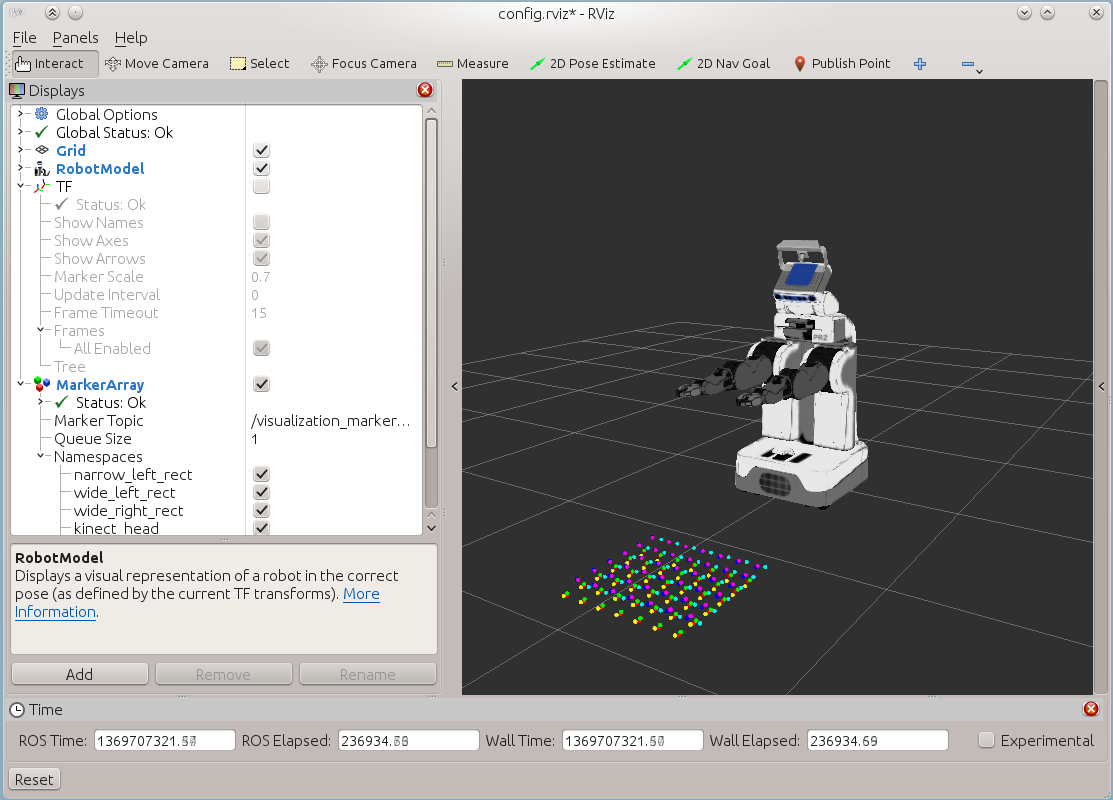
\includegraphics[width=0.7\textwidth]{images/screenshots/rviz.png}
 \caption{RViz interface.}
 \label{fig:rviz}
\end{figure}

\vspace*{-2ex}
\subsection{Roscpp}
\label{sec:roscpp}

Another primary ROS goal is \textit{``language independence''}: the ROS framework is easy to implement in any modern programming language, and it is already implemented in:
\begin{itemize*}
 \item Python (\url{http://www.ros.org/wiki/rospy}) and,
 \item C++ (\url{http://www.ros.org/wiki/roscpp}).
\end{itemize*}

\subsection{PR2}
\label{sec:PR2}

The PR2 (Personal Robot, version 2) is a Willow Garage which has two 7-DOF arms with a payload of 1.8 kilograms (1,800 g). Sensors include a 5 megapixel camera, a tilting laser range finder, and an inertial measurement unit. The ``texture projector'' projects a pattern on the environment to create 3D information for capture by the cameras. Also Microsoft Kinect can be head-mounted. In this work, its head (see left on Figure \ref{fig:pr2}) is the most important since all the cameras are located there and most be calibration to each other.
\begin{figure}[!htbp]
 \centering
 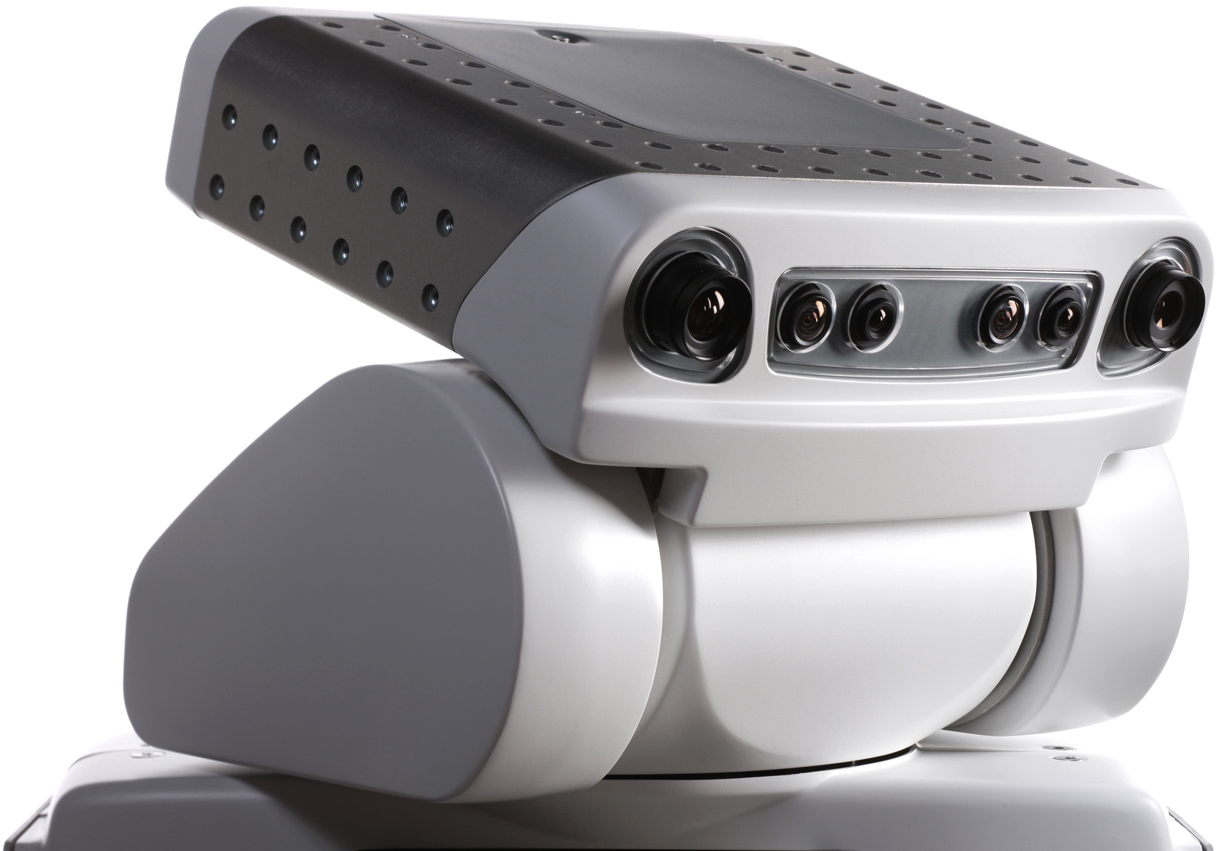
\includegraphics[width=0.45\textwidth]{images/PR2_01.jpg}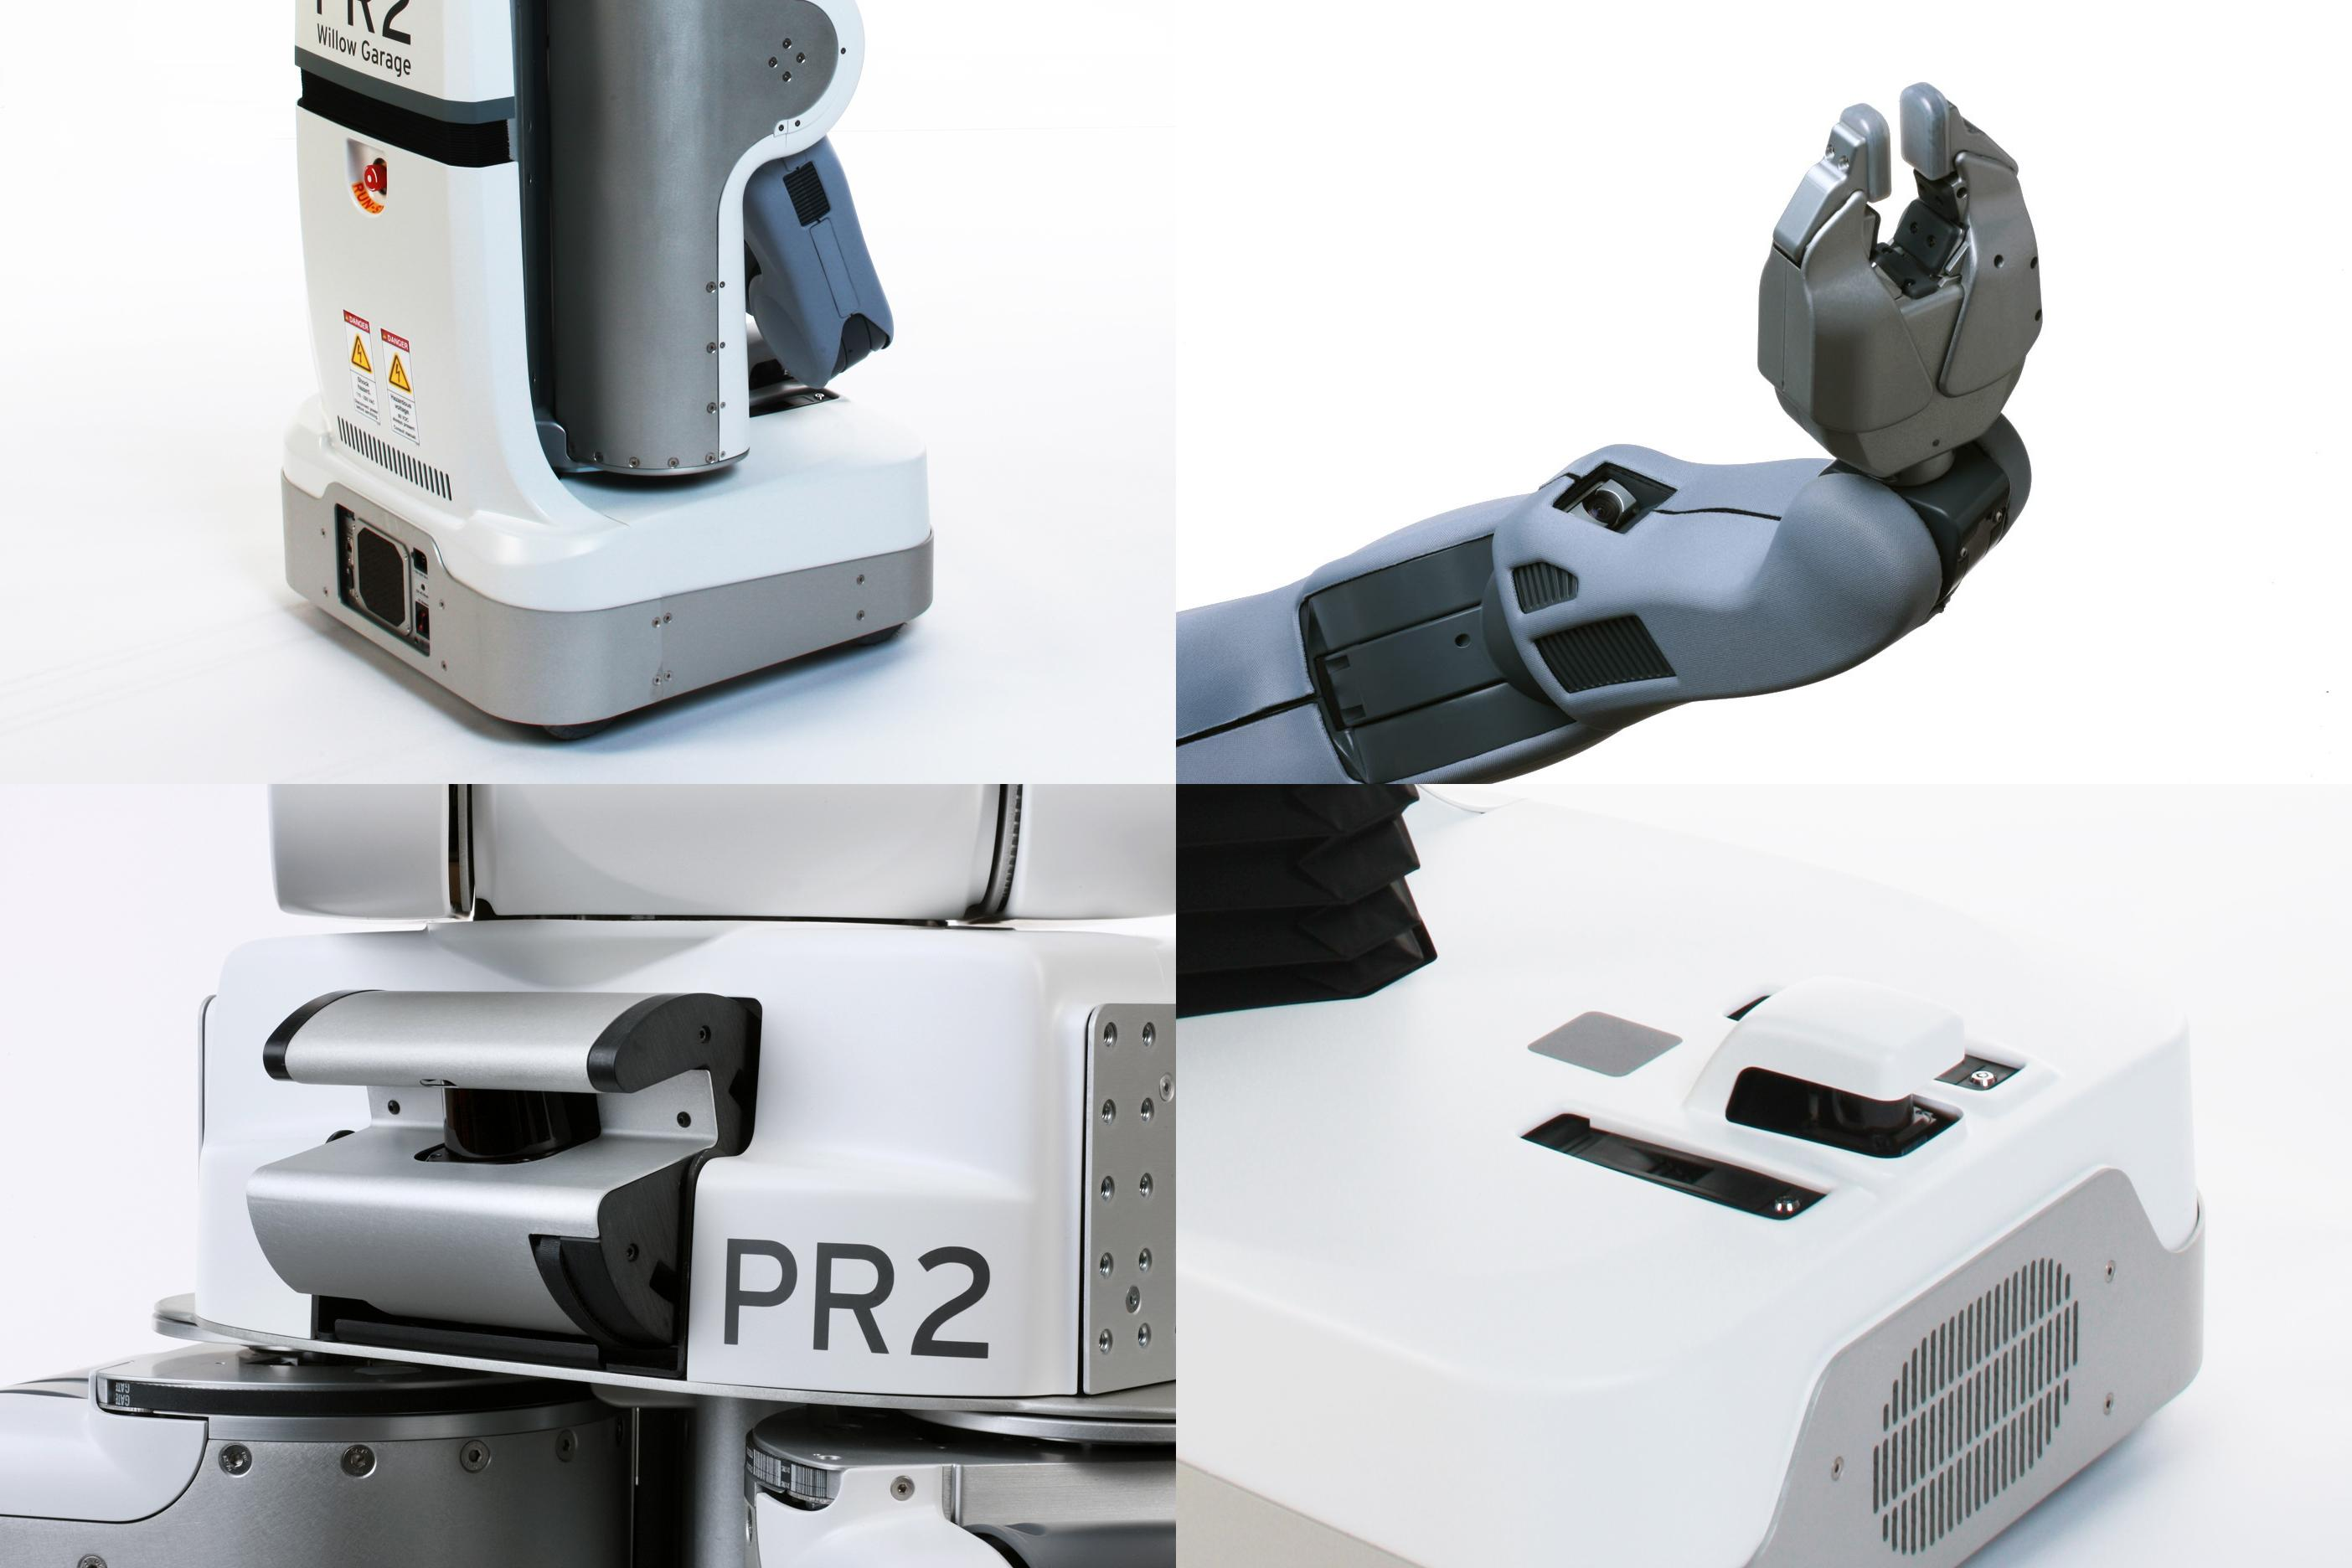
\includegraphics[width=0.45\textwidth]{images/PR2_joint.jpg}
 \caption{PR2 overview}
 \label{fig:pr2}
\end{figure}

\subsection{URDF}
\label{sec:urdf}

The URDF (\textbf{U}nified \textbf{R}obot \textbf{D}escription \textbf{F}ormat) is an XML format for representing a robot model. The package also contains a C++ parser, and it can be visualize with RViz (see in Figure~\ref{fig:pr2_urdf}).
For more information: \url{http://www.ros.org/wiki/urdf}.
\begin{figure}[!htbp]
 \centering
 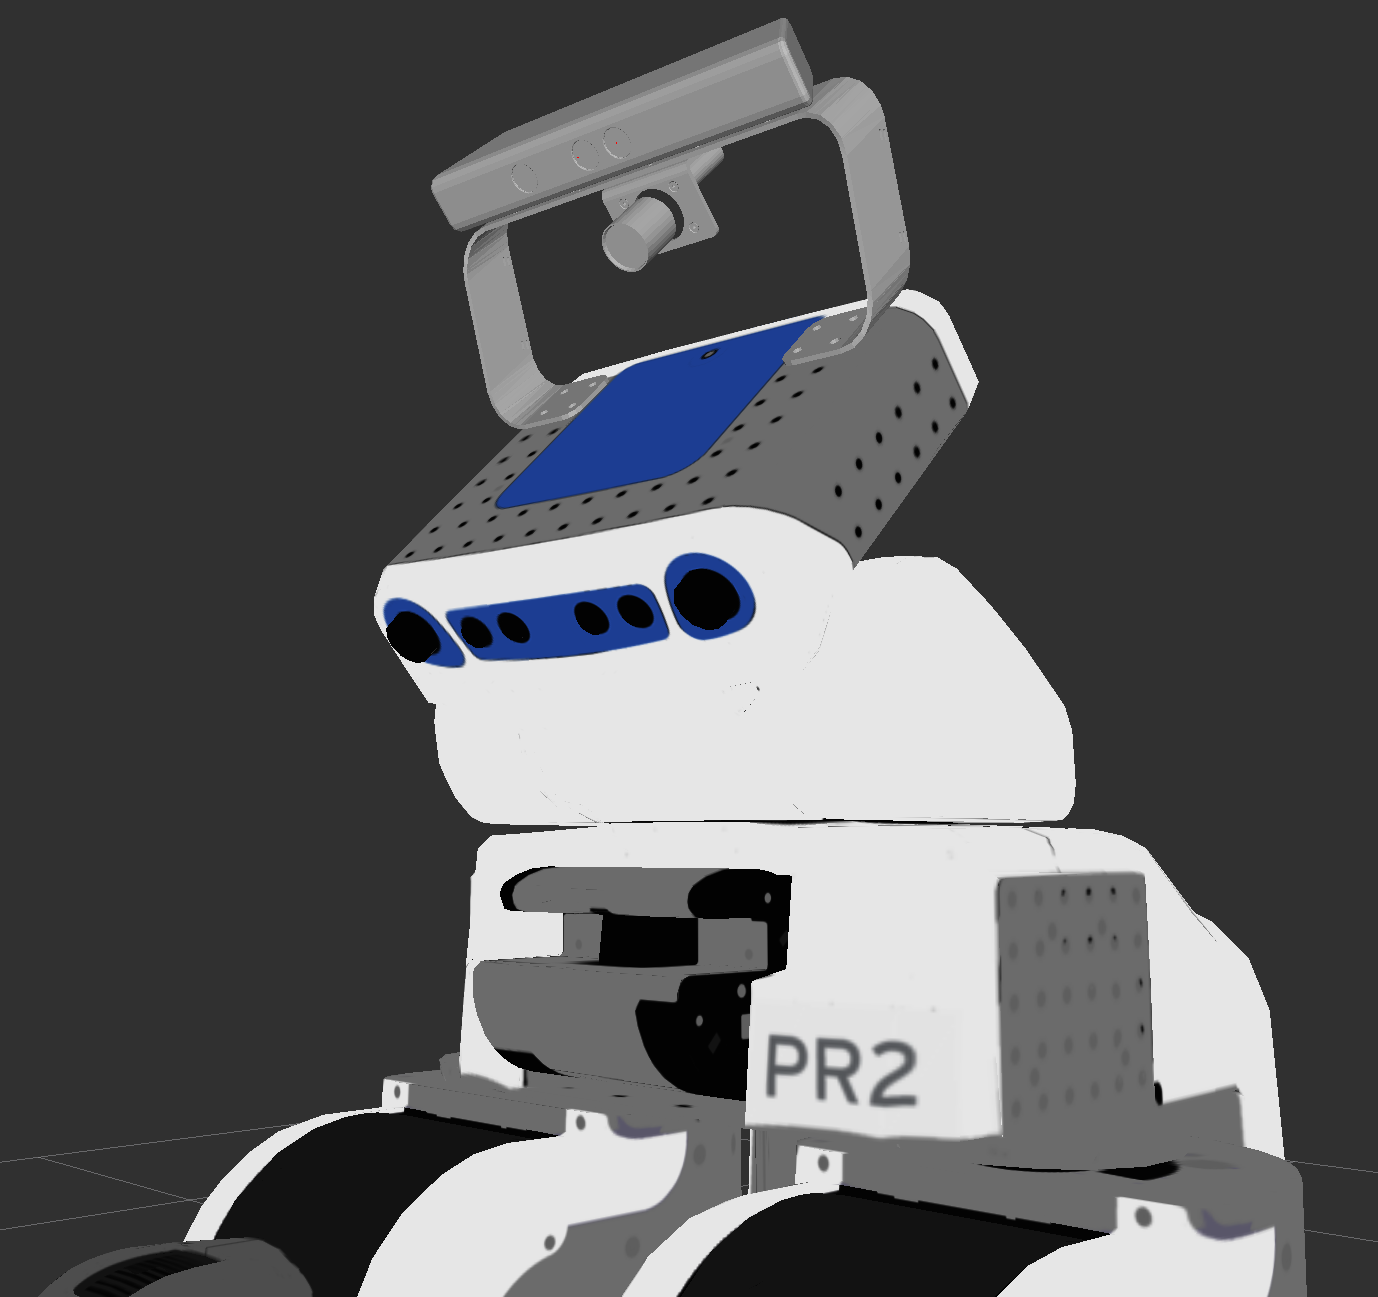
\includegraphics[width=0.35\textwidth]{images/screenshots/PR2_urdf.png}
 \caption{PR2 URDF model in RViz}
 \label{fig:pr2_urdf}
\end{figure}


\subsection{/tf}
\label{sec:tf}

The package /tf lets the user keep track of multiple coordinate frames over time. /tf maintains the relationship between coordinate frames in a tree structure buffered in time, and lets the user transform points, vectors, etc between any two coordinate frames at any desired point in time.

A robotic system typically has many 3D coordinate frames that change over time (see Figure~\ref{fig:tf}), such as a world frame, base frame, gripper frame, head frame, etc. /tf keeps track of all these frames over time.
For more information: \url{http://www.ros.org/wiki/tf}.

\begin{figure}[!htbp]
\centering
  \subfigure%[All coordinates system]
  {
    \centering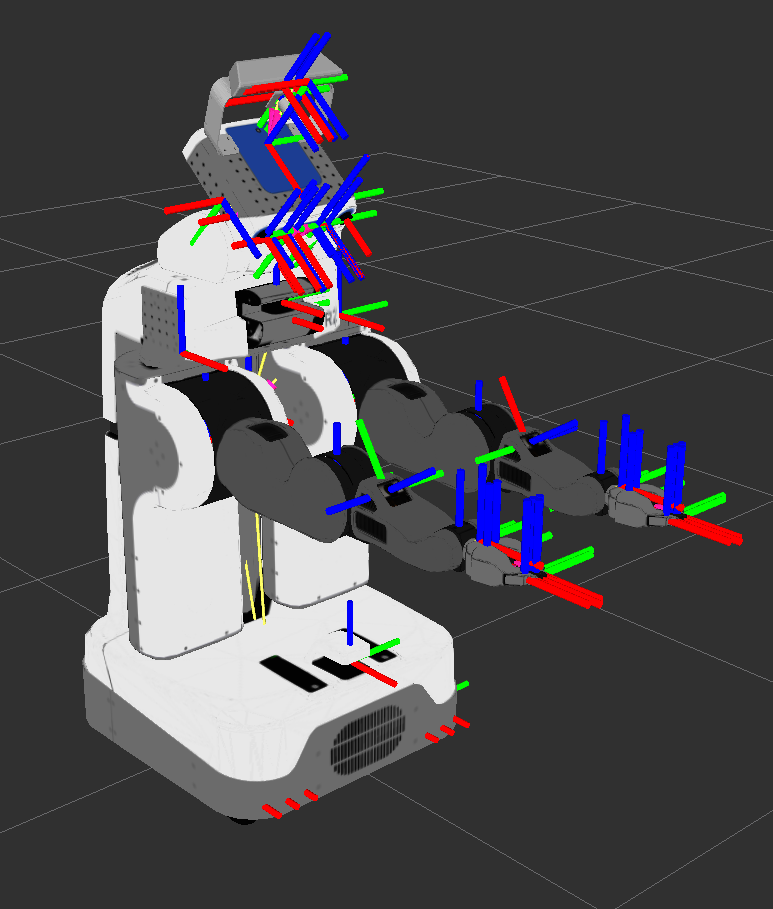
\includegraphics[height=0.3\textheight]{images/screenshots/tf01.png}
    \label{fig:tf01}
  }
  \subfigure%[\texttt{narrow\_stereo\_optical\_frame} until root]
  {
    \centering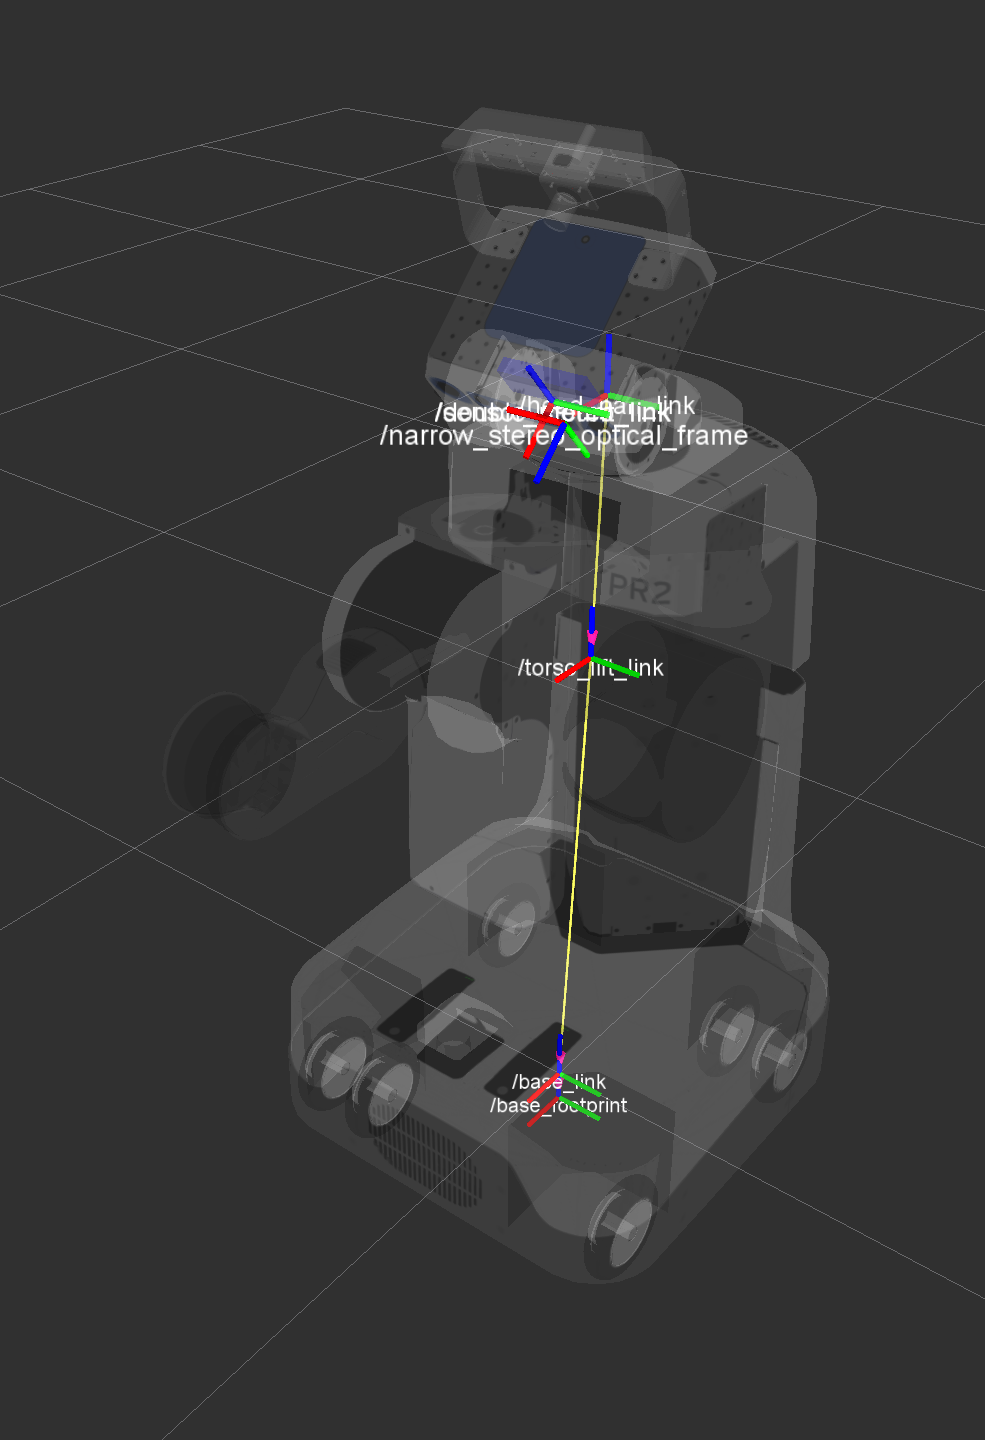
\includegraphics[height=0.3\textheight]{images/screenshots/tf02.png}
    \label{fig:tf02}
  }
  \caption{Example of /tf in RViz (in a particular time). On the left, all coordinates system; on the right, /tf path from \texttt{narrow\_stereo\_optical\_frame} until the robot root (\texttt{base\_footprint}).}
   \label{fig:tf}
\end{figure}


\subsection{ROS bag and rqt}
\label{sec:rosbag}

All the components for a simulated environment are implemented, and it is needed a way to reproduce events/messages. This is performed by ROS bag, which is a set of tools for recording from and playing back to ROS topics. It avoids deserialization and reserialization of the messages. More info: \url{http://www.ros.org/wiki/rosbag}.

\begin{figure}[!htbp]
 \centering
 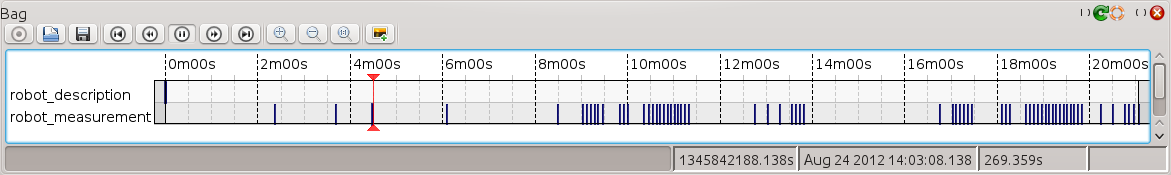
\includegraphics[width=0.95\textwidth]{images/screenshots/rosbag01.png}
 \caption{rqt: \rosbag~interface.}
 \label{fig:rosbag01}
\end{figure}

A second tool described here is a rqt plugin which allows to play a ROS bag easily (Figure~\ref{fig:rosbag01}). The user will be able to see the ROS messages in a convenient way (Figure~\ref{fig:rosbag02}). More info: \url{http://www.ros.org/wiki/rqt}.

\begin{figure}[!htbp]
 \centering
 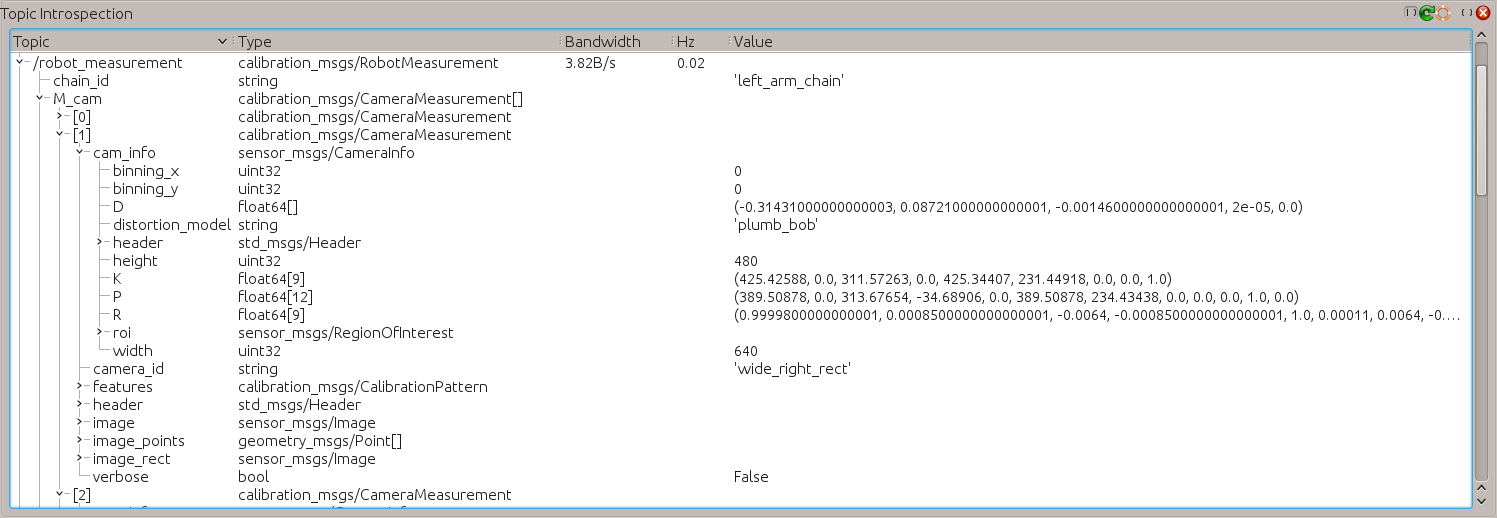
\includegraphics[width=0.95\textwidth]{images/screenshots/rosbag02.png}
 \caption{rqt: Topic introspection.}
 \label{fig:rosbag02}
\end{figure}

\subsection{Image\_proc\_node}

The node \texttt{image\_proc} sit between the camera driver and vision processing nodes (see Figure \ref{fig:img_proc02}). \texttt{image\_proc} removes camera distortion from the raw image stream, and if necessary will convert Bayer or YUV422 format image data to color

\begin{figure}[!htbp]
 \centering
 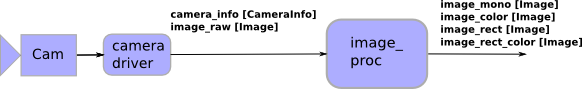
\includegraphics[width=0.7\textwidth]{images/img_proc02.png}
 \caption{De-mosaics and undistorts the raw camera image stream.}
 \label{fig:img_proc02}
\end{figure}

% \noindent
All processing is on demand. Color processing is performed only if there is a subscriber to a color topic. Rectification is performed only if there is a subscriber to a rectified topic. While there are no subscribers to output topics, \texttt{image\_proc} unsubscribes from the \texttt{image\_raw} and \texttt{camera\_info} topics.

More info: \url{http://www.ros.org/wiki/image_proc}.


\subsection{Camera model in ROS}

Figure \ref{fig:camera_model02} is a diagram of the camera coordinate system assumed. It is a right-handed system, with the world X and Y aligned with the image x and y.

The camera model used in ROS is the same coordinate system used in OpenCV. It differs from the coordinate system of Harley and Zisserman in \cite{HZ2}, which has Z forward, Y up, and X to the left (looking towards +Z).

\begin{figure}[!htbp]
 \centering
 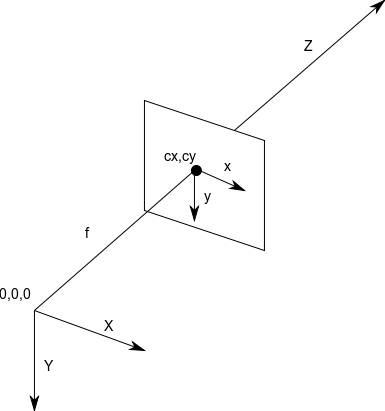
\includegraphics[width=0.35\textwidth]{images/camera_model02.png}
 \caption{The camera coordinate system assumed.}
 \label{fig:camera_model02}
\end{figure}

More info: \url{http://www.ros.org/wiki/image_pipeline/CameraInfo}.

\subsubsection{Derivation diagram}

Figure \ref{fig:camera_model03} is a diagram of the various images that are conceptually derivable from the CameraInfo message\footnote{CameraInfo message is a ROS message where all the camera information is saved.}. The boxed variables are present in this message.

\begin{figure}[!htbp]
 \centering
 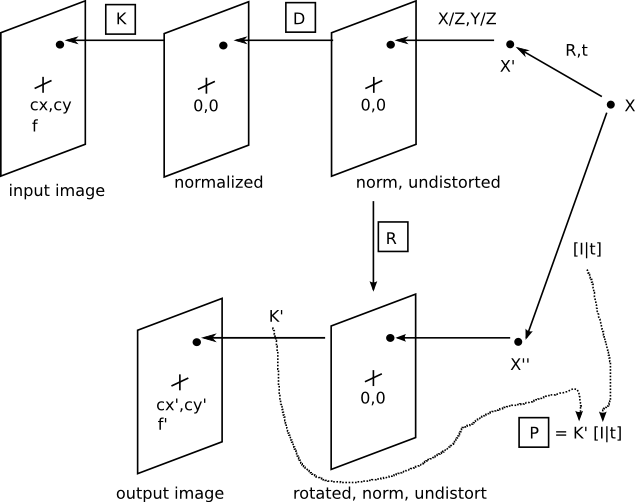
\includegraphics[width=0.75\textwidth]{images/camera_model03.png}
 \caption{Derivation diagram}
 \label{fig:camera_model03}
\end{figure}

\subsubsection{Projection onto the original image}

Starting with an initial 3D point $X$, the position of the corresponding image point is found by going right-to-left in the upper half of the diagram \ref{fig:camera_model03}. The process is summarized by the following equations:
\[
\begin{array}{rcll}
X' &=& [R,t]\,X  & \quad \quad \texttt{transform} \\
sx &=& X'        & \quad \quad \texttt{projection} \\
x* &=& d(x)      & \quad \quad \texttt{distortion} \\
q  &=& Kx*       & \quad \quad \texttt{pixel coordinates}
\end{array}
\]
This process uses the $K$ camera matrix and $D$ distortion vector. Ignoring the transform $T$, the projection of a point $X$' can be found into the original camera frame using these equations. First, the $3D$ point $X$' is projected onto the normalized, undistorted image via a projection operation (division by $Z$). Then the distortion coefficients are used in the function $d()$ to move the point to its distorted position, still in a normalized image. Finally, the normalized image is converted to a pixel-coordinate image by applying the camera matrix to each image point.


\subsubsection{Rectification}
\label{sec:rectification}
In this context, rectification is the process of transforming the input image into an output image with the distortion corrected (Figure \ref{fig:camera_model03}), and optionally transformed by rotation, in-plane translation, and scale.

In the case of a \textbf{monocular rectification} with distortion correction, to transform a pixel in the input image into one in the output image, it is sent through the $K - D - R - K'$ series of transformations. $K - D$ gets to the normalized, undistorted image; the rotation $R$ is the identity because we don't want to rotate the image; and then $K'$ converts back to pixel coordinates in the output image. In this case, since there is no rotation, translation, or scaling from the original image, $K = K'$ , and only the $K$ and $D$ elements of CameraInfo are needed.
An example of this process can be seen in Figure \ref{fig:rectification}.
\begin{figure}[!htbp]
\centering
  \subfigure[\textbf{image\_raw}: original camera image, Bayered and distorted]
  {
    \centering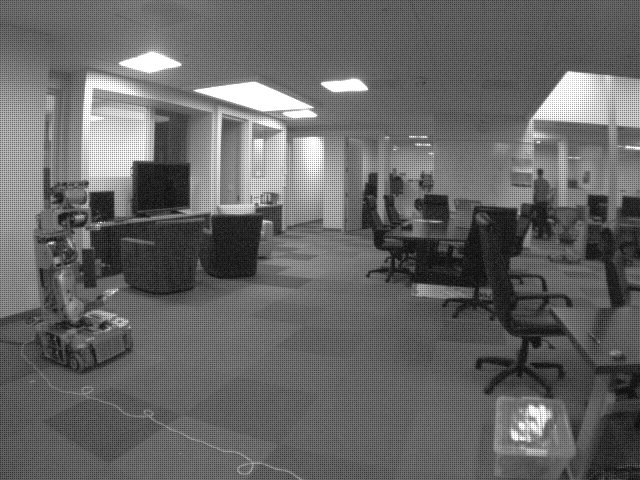
\includegraphics[height=0.25\textheight]{images/img_proc_left_raw.png}
    \label{fig:img_proc_left}
  }
  \subfigure[\textbf{image\_rect}: rectified image, de-Bayered and undistorted (amount of black border may vary depending on calibration)]
  {
    \centering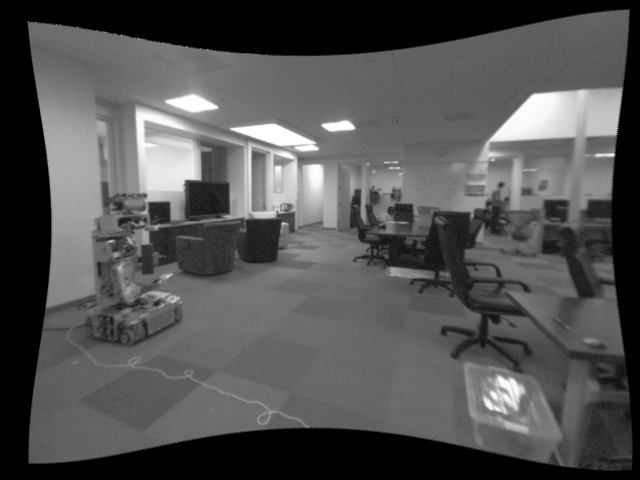
\includegraphics[height=0.25\textheight]{images/img_proc_rectified.png}
    \label{fig:img_proc_rect}
  }
  \caption{Rectification (and de-Bayer) process performed by \texttt{\texttt{image\_proc}\_node}.}
   \label{fig:rectification}
\end{figure}



\section{KDL}
\label{sec:KDL}

KDL (\textbf{K}inematics and \textbf{D}ynamics \textbf{L}ibrary) defines a tree structure to represent the kinematic and dynamic parameters of a robot mechanism (see Figure \ref{fig:KDL}). \textit{kdl\_parser} provides tools to construct a KDL tree from an XML robot representation in URDf format.

\begin{figure}[!htbp]
 \centering
 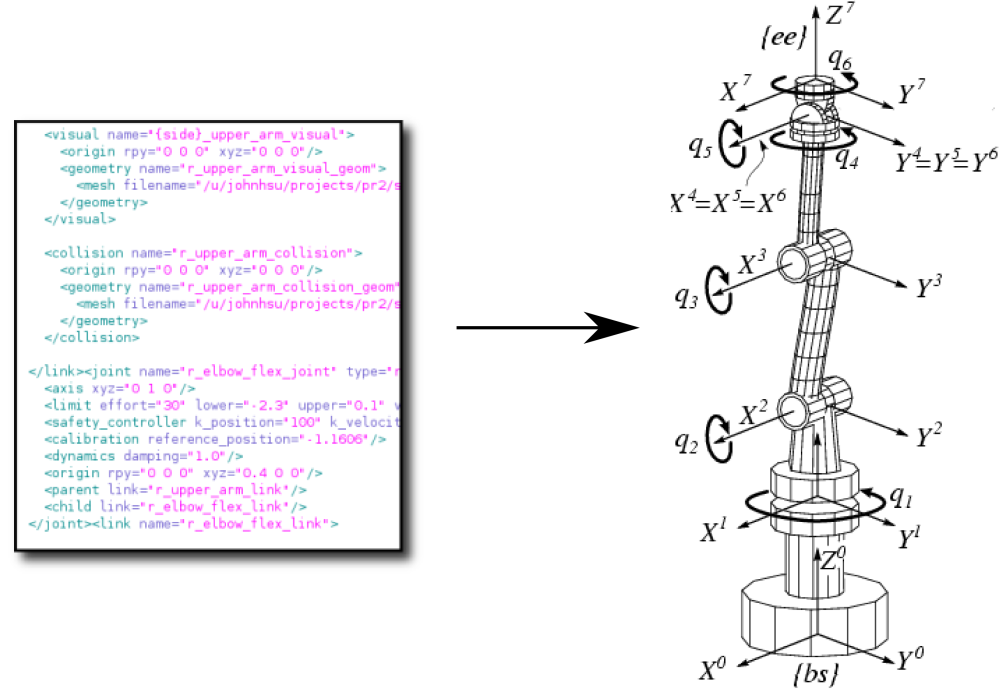
\includegraphics[width=0.7\textwidth]{images/KDL02.png}
 \caption{Example of KDL tree.}
 \label{fig:KDL}
\end{figure}

This library is mainly used for:
\begin{itemize*}
 \item 3D frame and vector transformations,
 \item forward kinematics (given joint angles compute the position of the end-effector\footnote{An \textit{end-effector} is the device at the end of a robotic arm, designed to interact with the environment, in our case the cameras.}).
\end{itemize*}


For more information: \url{http://www.ros.org/wiki/kdl}.

\section{Ceres}
\label{sec:ceres}

Ceres Solver \cite{ceres} is a portable C++ library that allows modeling and solving large complicated \textbf{non-linear least squares} problems. It is used at Google to estimate the pose of Street View cars, aircrafts, and satellites; to build 3D models for PhotoTours; to estimate satellite image sensor characteristics, and more.

Ceres Solver is an important component in this thesis because it has very good features like, among others:
\begin{itemize*}
\item A friendly API: build your objective function one term at a time.
\item Automatic Analytic Derivatives.
\item Specialized solvers for bundle adjustment problems in computer vision.
% \item Iterative linear solvers for general sparse and bundle adjustment problems.
\end{itemize*}

It will too long to make a good introduction to Ceres, but a briefly description of important points, obtained from the tutorial, can be found in the following. The excellent tutorial is available in: \url{http://homes.cs.washington.edu/~sagarwal/ceres-solver/tutorial.html}.

\subsection*{Modeling}
Ceres solves robustified non-linear least squares problems of the form:
\begin{equation}
\frac{1}{2}\sum_{i=1} \rho_i\left(\left\|f_i\left(x_{i_1}, ... ,x_{i_k}\right)\right\|^2\right).
\end{equation}

The expression $\rho_i\left(\left\|f_i\left(x_{i_1},...,x_{i_k}\right)\right\|^2\right)$ is known as a \texttt{ResidualBlock}, where $f_i(\cdot)$ is a \texttt{Cost Function} that depends on the parameter blocks $\left[x_{i_1},... , x_{i_k}\right]$. In most optimization problems small groups of scalars occur together. For example, the three components of a translation vector and the four components of the quaternion that define the pose of a camera. Such groups of small scalars are called \texttt{ParameterBlock}.

$\rho_i$ is a \texttt{LossFunction}. A \texttt{LossFunction} is a scalar function that is used to reduce the influence of outliers on the solution of non-linear least squares problems. As a special case, when $\rho_i(x) = x$, i.e., the identity function, it leads to the more familiar non-linear least squares problem.
\[
 \frac{1}{2}\sum_{i=1} \left\|f_i\left(x_{i_1}, ... ,x_{i_k}\right)\right\|^2.
\]

\subsection*{Derivatives}
Ceres Solver like most optimization packages, depends on being able to evaluate the value and the derivatives of each term in the objective function at arbitrary parameter values. Doing so correctly and efficiently is essential to getting good results. Ceres Solver provides a number of ways of doing so: Analytic and Numeric Derivatives. In order to use Automatic differentiation, it is necessary to define a \textbf{templated} cost functor\footnote{A functor is a class with an \texttt{operator()} member. And a cost functor is a functor which evaluate the residuals.}.



\section{OpenCV}

OpenCV is integrated in ROS and used in many parts of this thesis, in special the function called solvePnP and Rodrigues's formula detailed next.


\subsection{Rodrigues' formula}

Converts a rotation matrix to a rotation vector\footnote{This is an axis-angle representation, an using the vector module as the angle that describe the magnitude of the rotation about the axis.} and vice versa. A rotation vector is a convenient and most compact representation of a rotation matrix (since any rotation matrix has just 3 degrees of freedom).

\begin{figure}[!htbp]
 \centering
 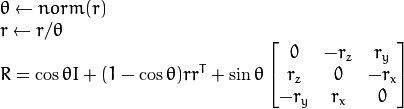
\includegraphics[width=0.5\textwidth]{images/rodrigues01.png}
 \caption{Rodrigues' formula}
 \label{fig:rodrigues}
\end{figure}

% More info: \url{http://docs.opencv.org/modules/calib3d/doc/camera_calibration_and_3d_reconstruction.html#rodrigues}.



\subsection{SolvePnP}
\label{sec:solvePnP}

Without loss of generality, it is assumed the model plane (i.e., a checkerboard) is on $Z=0$ of the world coordinate system. Let's denote the $i^{th}$ column of the rotation matrix $R$ by $r_i$. From~(\ref{eq:pinhole}),
\begin{equation}
  s\,\begin{pmatrix}
      x \\
      y \\
      1
\end{pmatrix}
= K\, [r_1~~r_2~~r_3~~t]\,\begin{pmatrix}
      X \\
      Y \\
      0 \\
      1
\end{pmatrix}
= K\, [r_1~~r_2~~t]\begin{pmatrix}
      X \\
      Y \\
      1
\end{pmatrix}
\end{equation}
Therefore, a model point $\mathbf{X}$ and its image $\mathbf{x}$ are related by a homography; and this can be used for solvePnP (see more details in the implementation chapter \ref{sec:solvePnP_impl}).

More precisely, SolvePnP give a solution to the \textbf{PnP problem} --the estimation of the pose of a calibrated camera from $n$ 3D-to-2D point correspondences-- minimizing the reprojection error. In others words, it finds the rotation and translation from the checkerboard coordinate system to the camera coordinate system.

% More info: \url{http://docs.opencv.org/modules/calib3d/doc/camera_calibration_and_3d_reconstruction.html#solvepnp}


% \subsection{Camera model with distortion}
%
% %TODO
% ( I will might delete this section since I don't use distortion!! )
%
% ROS uses the same the camera model with distortion than OpenCV, see in Figure~\ref{fig:camera_model_opencv}.
%
% \begin{figure}[!htbp]
%  \centering
%  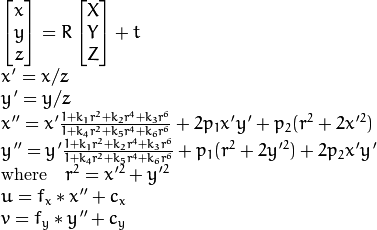
\includegraphics[width=0.45\textwidth]{images/camera_model_opencv.png}
%  \caption{OpenCV Camera model with distortion}
%  \label{fig:camera_model_opencv}
% \end{figure}
%




